\documentclass[final]{beamer}
%% based on the Dreuw style
\mode<presentation>
{
\setbeamertemplate{block begin}{
  \vskip.25ex
  \begin{beamercolorbox}[rounded=true,shadow=true,leftskip=1cm,colsep*=.75ex]{block title}%
    \usebeamerfont*{block title}\insertblocktitle
  \end{beamercolorbox}%
  {\ifbeamercolorempty[bg]{block body}{}{\nointerlineskip\vskip-0.5pt}}%
  \usebeamerfont{block body}%
  \begin{beamercolorbox}[rounded=true,shadow=false,colsep*=.75ex,sep=.75ex,vmode]{block body}%
    \ifbeamercolorempty[bg]{block body}{\vskip-.25ex}{\vskip-.75ex}\vbox{}%
  }
  \setbeamertemplate{block end}{
  \end{beamercolorbox}
}
\setbeamertemplate{headline}{
  \leavevmode

  \begin{beamercolorbox}[wd=\paperwidth]{headline}
    \begin{columns}[T]
      \begin{column}{.02\paperwidth}
      \end{column}
      \begin{column}{.22\paperwidth}
        \begin{center}
         
\includegraphics[scale=0.1]{transparentStatisticsLaura201617.jpg}
         
\includegraphics[scale=0.16]{nsf.png}
        \end{center}
        \vskip0.5ex
      \end{column}
      \begin{column}{.675\paperwidth}
        \vskip4ex
        \raggedleft
        \usebeamercolor{title in headline}{\color{fg}\textbf{\LARGE{\inserttitle}}\\[1ex]}
        \usebeamercolor{author in headline}{\color{fg}\large{\insertauthor}\\[1ex]}
        \usebeamercolor{institute in headline}{\color{fg}\large{\insertinstitute}\\[1ex]}
      \end{column}
      \begin{column}{.1\paperwidth}
        \vskip1cm
        \begin{center}
          
\includegraphics[scale=0.5]{Purduelogo.jpg}
        \end{center}
        \vskip1.5cm
      \end{column}
      \begin{column}{.03\paperwidth}
      \end{column}
    \end{columns}
  \end{beamercolorbox}

  \begin{beamercolorbox}[wd=\paperwidth]{lower separation line head}
    \rule{0pt}{2pt}
  \end{beamercolorbox}
}
}
\usecolortheme{purduegold}
\usepackage{times}
\usepackage{tikz}
\usepackage{pgfplots}
\pgfplotsset{compat=1.5}
\usetikzlibrary{calc}
\usepackage{amsmath,amsthm, amssymb, latexsym}
\boldmath
\usepackage[english]{babel}
\usepackage[latin1]{inputenc}
\usepackage[size=custom,width=101,height=76, scale=1,debug]{beamerposter}

\usepackage[round]{natbib}
\usepackage{graphicx}
\usepackage{url}
\usepackage{bm}

\usepackage{lipsum}  

\graphicspath{{figures/}}
  \title[Fancy Posters]{Rates of DNA Mutation in Genes and Inte-Gene Regions}
  \author{Laszlo Csonka, Mark Daniel Ward, Brian French, and Nicole Markley}
  \institute{Department of Biology, Purdue University, West Lafayette, IN}
%  \date{March 25, 2016}

  \begin{document}
  \begin{frame}{}
    \begin{columns}[t]

%%%%%%%%%%%%%%%%%%%%%%%%%%%%%%%%%%%%%%%%%%%%%%%%%%%%%%%%%%%%%%%%%%%%%%

    \begin{column}{.32 \linewidth}
    \begin{block}{\large Abstract}
The aim of our analysis was to compare the rates of evolution of DNA sequences of genes and intergenic regions. The chromosomes of the related genera of bacteria, Escherichia coli K-12, Salmonella enterica serovar Typhimurium, and Citrobacter koseri, contain extensive regions in which the order of genes of identical. The fact that the gene order is so conserved suggests that both the genes and intergenic spacers were derived by evolution from corresponding sequences in the last common ancestor of the three organisms, and it enabled us to compare the sequence changes in functional genes and in intergenic spacers across the three organisms.
\newline
\newline
Pairwise comparisons using BLASTN were used to identify regions that had shared genes. ClustalW was then used to identify single base mutations in both genes and inter-gene regions. Mutation frequencies were determined for all paired comparisons. This analysis indicated that the mutation frequencies are significantly higher in intergenic spacers do not have specific sequence-dependent functions, and therefore, they can accumulate mutations more liberally than genes, which are constrained by their function.
    \end{block}

\begin{block}{\large Introduction}
Genomes have both useful genetic information and presumed useless inter-gene regions termed as gaps. Gene pairs between organisms can be isolated using a tool called \textbf{B}asic \textbf{L}ocal \textbf{A}lignment \textbf{S}earch \textbf{T}ool, commonly referred to as BLAST. 

\newline
\textit{Salmonella Typhimurium LT2}, \textit{Citrobacter Koseri}, and \textit{Escherchia Coli MG1655} were chosen because Dr. Csonka told me to use them--add real reason later
\end{block}

 \begin{block}{\large Motivation}
Mutation in genes has a double constrainment of DNA's built in error-handling as well as maintaining function. We suspected that looking at both genes and gaps it could be determined how much similarity there would be in accumulation of mutations at the base level.
	\end{block}

 \begin{block}{\large Research Question}
	{\color{red} We want to characterize something. }
                       The end.
                       \newline
                       TL;DR: Do mutations happen in genes and gaps at the same rate?
	\end{block}

\end{column}

%%%%%%%%%%%%%%%%%%%%%%%%%%%%%%%%%%%%%%%%%%%%%%%%%%%%%%%%%%%%%%%%%%%%%%

\begin{column}{.32 \linewidth}

\begin{block}{\large Illustrations}
Put some ideas here, to tell about the ideas.
	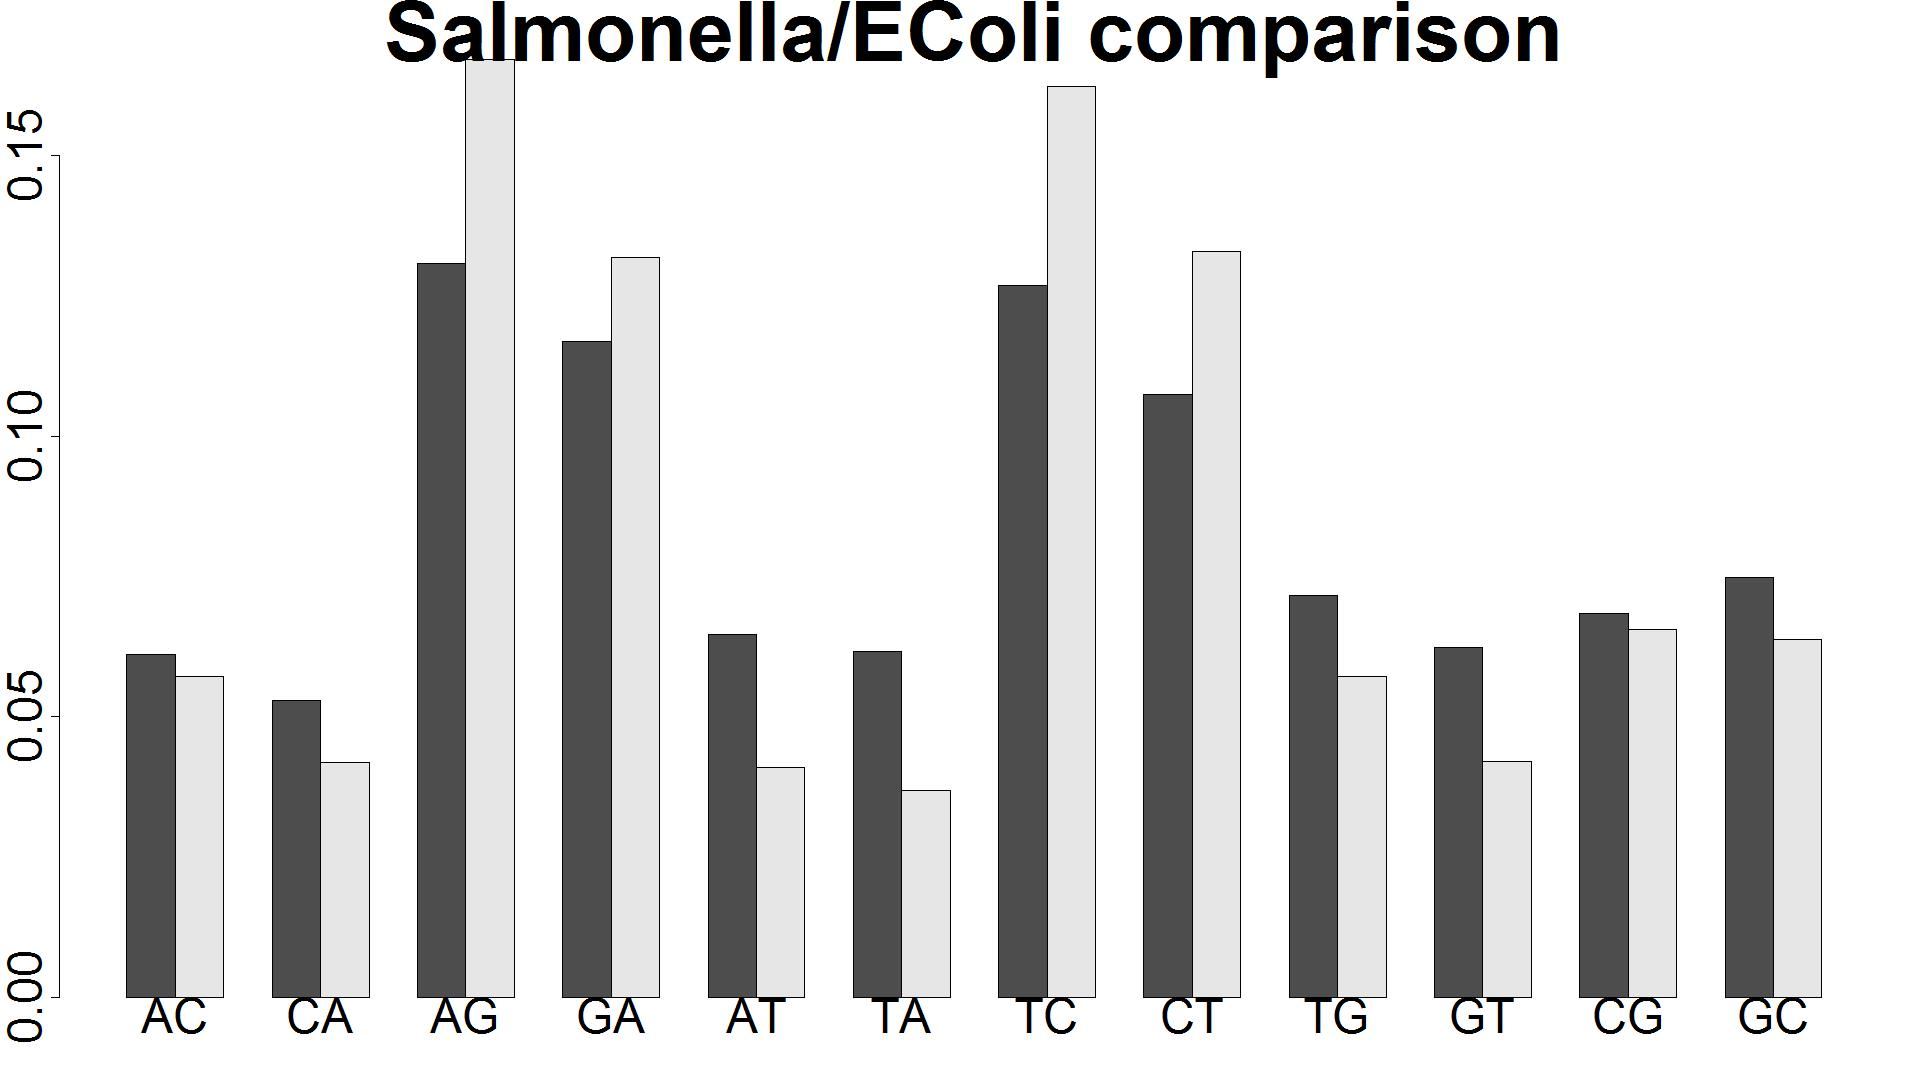
\includegraphics[scale = .455]{SalECPercentage.jpeg}
	\newline
 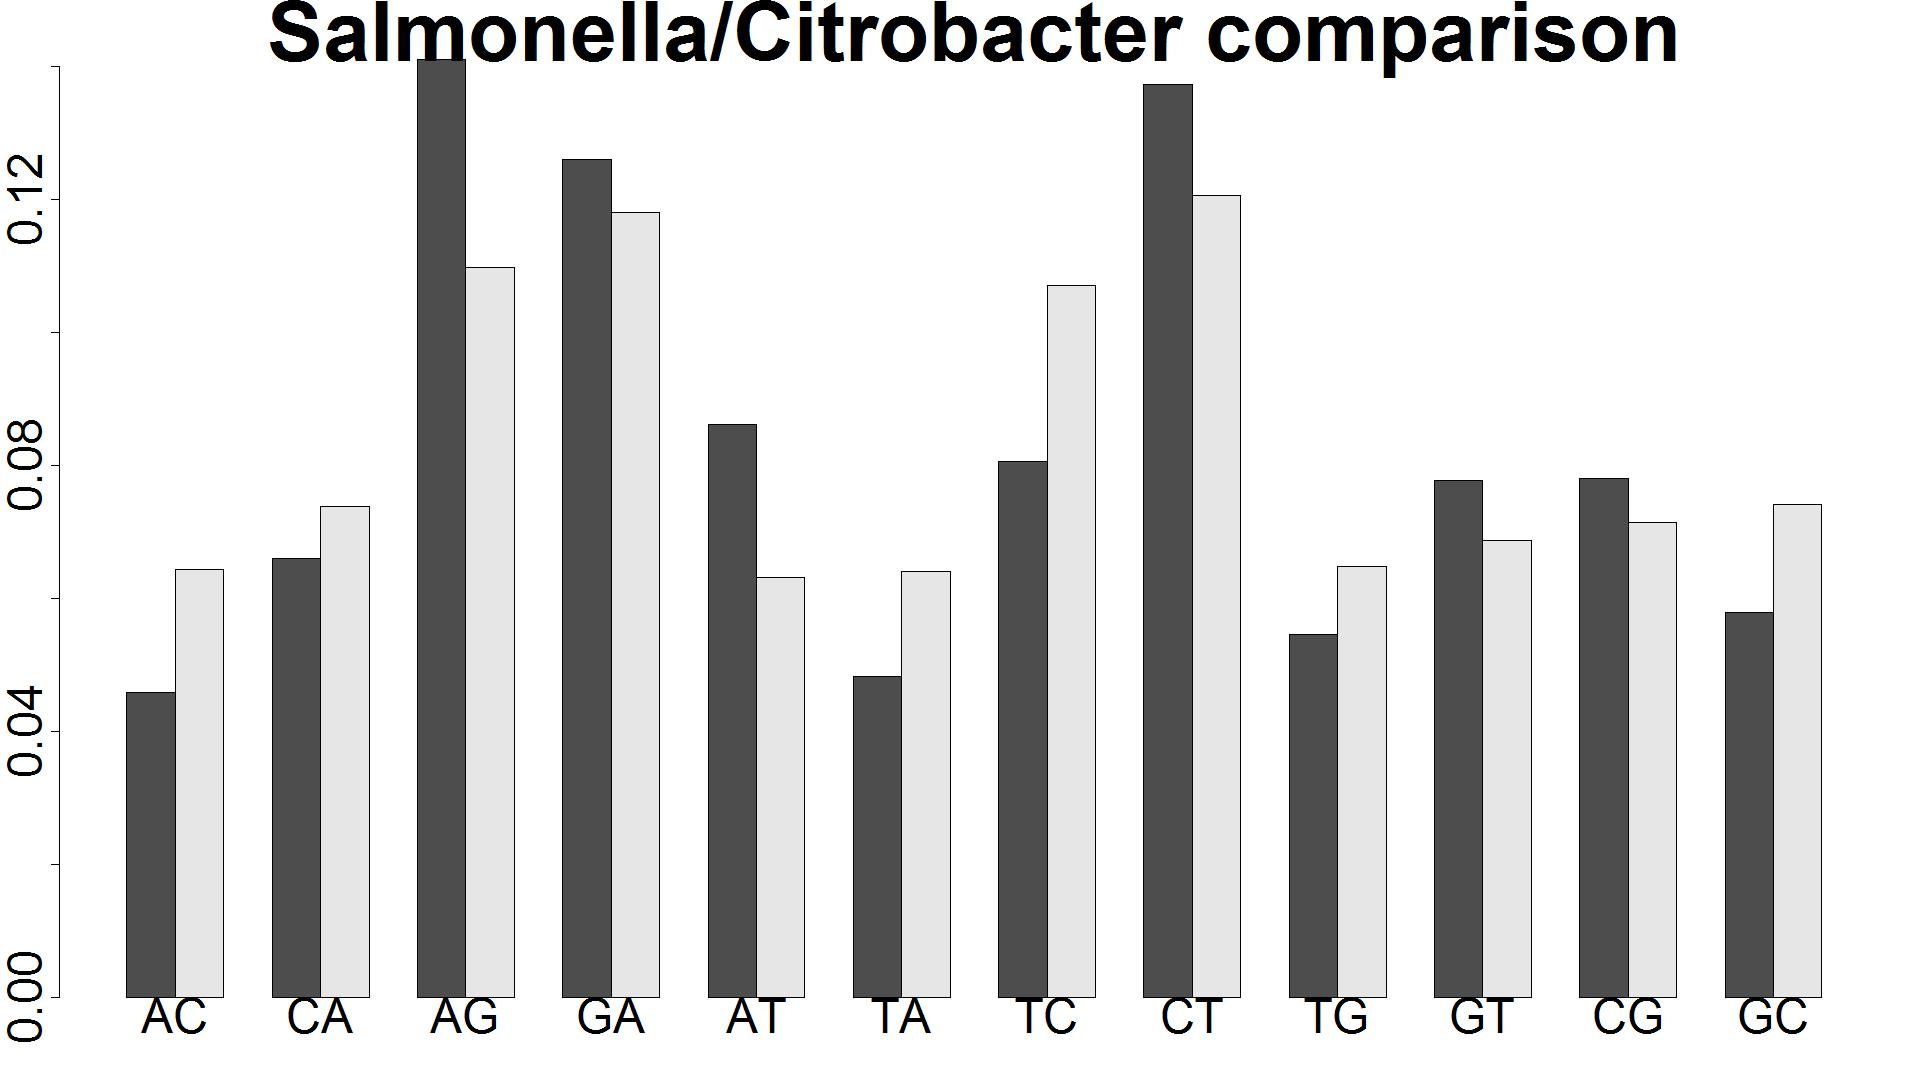
\includegraphics[scale = .455]{CBSalPercentage.jpeg}
 \newline
 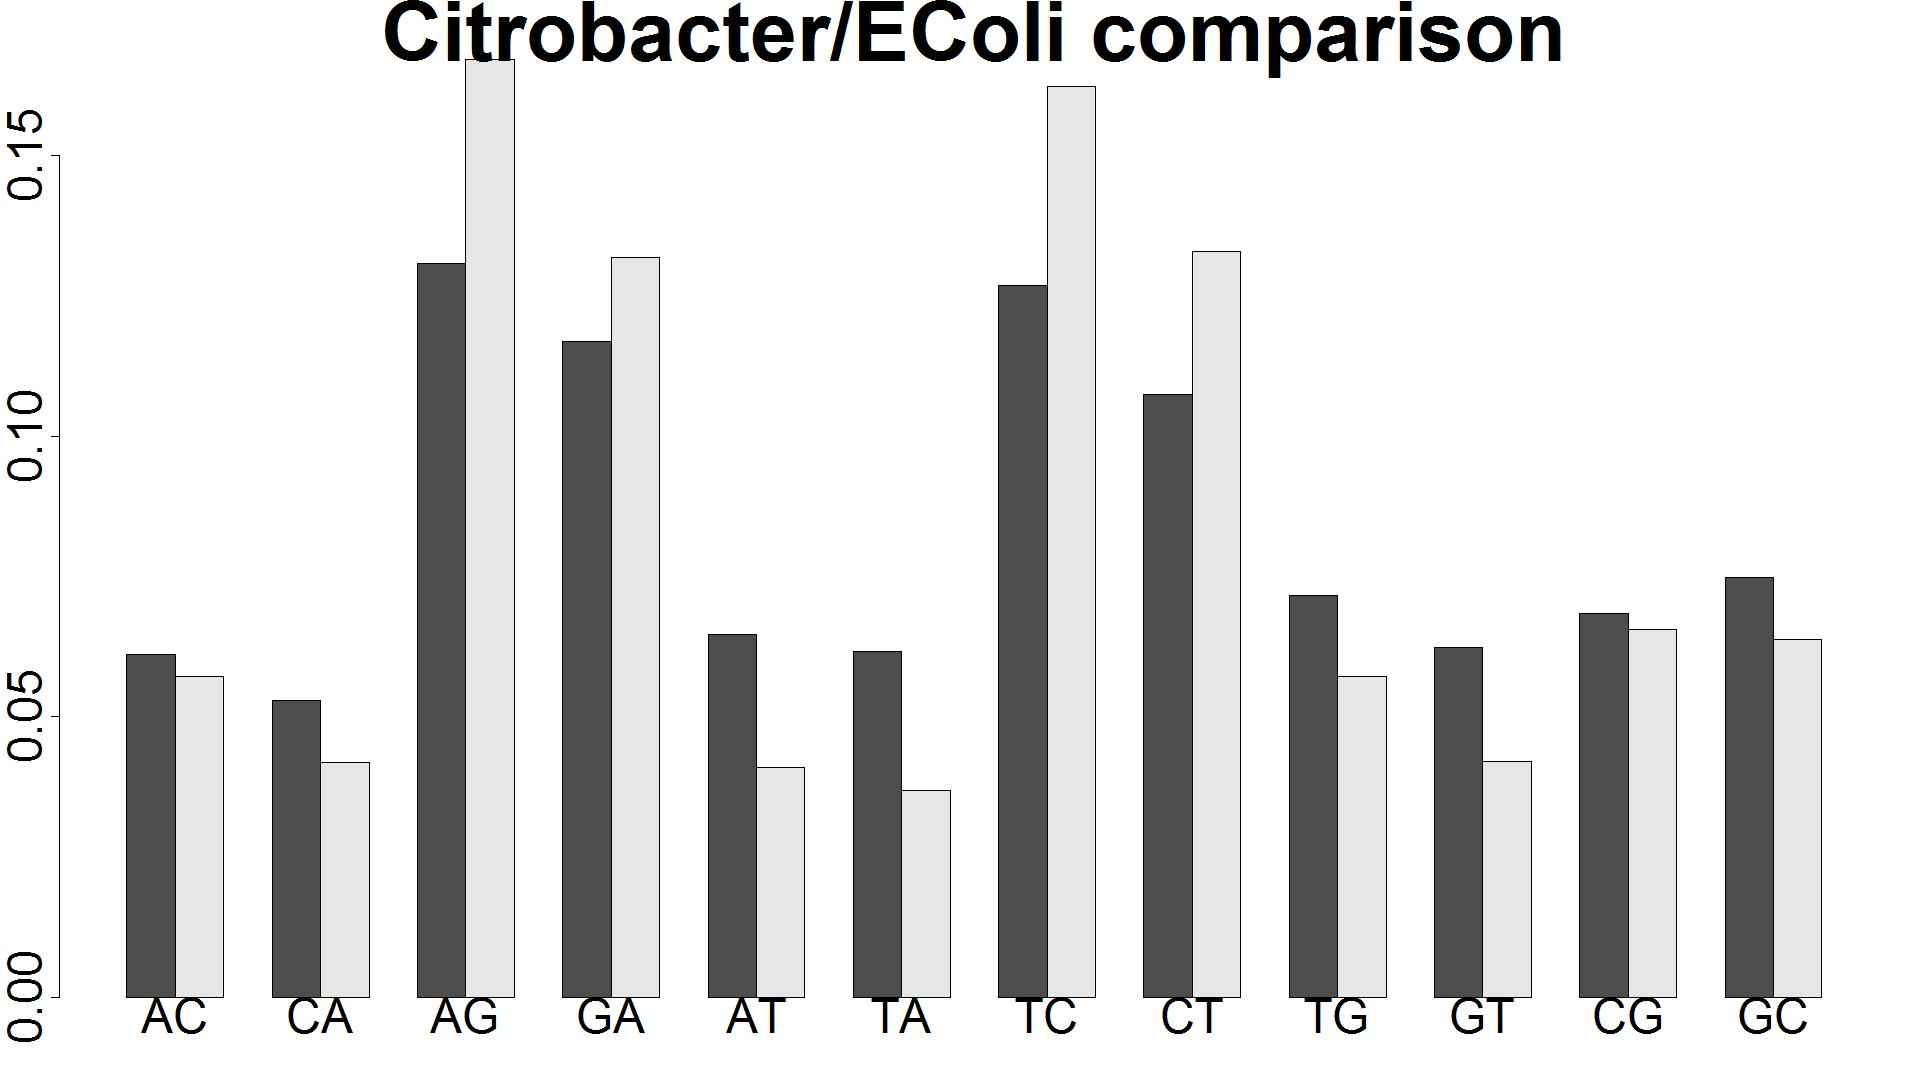
\includegraphics[scale = .455]{CBECPercentage.jpeg}
                       The end.

\end{block}

\begin{block}{\large Example}
  This just states an example about the research.
  It might be nice to add a pretty picture here.
\end{block}

\begin{block}{\large Application}
  Now I can discuss why that result matters to people.
\end{block}

\end{column}



%%%%%%%%%%%%%%%%%%%%%%%%%%%%%%%%%%%%%%%%%%%%%%%%%%%%%%%%%%%%%%%%%%%%%%

\begin{column}{.32 \linewidth}

\begin{block}{\large Conclusion}
Put some concluding remarks here

                         \lipsum[7-12] % This generates extra text!

\end{block}


%%% If you know how to use BibTeX
%%%	  \begin{block}{\large References}
%%%	  \vspace{-.5cm} \footnotesize
%%%	\bibliographystyle{abbrvnat}     % mathematics and physical sciences
%%%	\bibliography{forbidden}   % name your BibTeX data base
%%%	\vspace{-.25cm}
%%%	 \end{block}
	
	  \begin{block}{Acknowledgments}
The research of Student Name is supported by NSF grant DMS \#1246818.
Other thoughts can be placed here.
	 \end{block}



        \end{column}

    \end{columns}

  \end{frame}
\end{document}



